\documentclass[12pt,a4wide]{report}
\usepackage{amsthm,amssymb,mathrsfs,setspace,pstcol,textcomp,amsmath}
\usepackage{amsmath}
\usepackage{setspace}
\usepackage{epsfig}
\usepackage{geometry}    
\usepackage{graphicx}
\usepackage{graphics}
%\usepackage{comment}
\usepackage{float}
\restylefloat{figure}
%\usepackage[active]{srcltx}
%\usepackage[notcite,notref,color]{showkeys}
%\usepackage{epstopdf}
%\usepackage{graphicx, subfigure}
%\usepackage{epsfig}
\renewcommand{\chaptermark}[1]{\markboth{#1}{}}
\renewcommand{\sectionmark}[1]{\markright{\thesection\ #1}}


\input xy
\xyoption{all}


\theoremstyle{plain}
\newtheorem{theorem}{Theorem}[section]
\newtheorem{lemma}[theorem]{Lemma}
\newtheorem{corollary}[theorem]{Corollary}
\newtheorem{proposition}[theorem]{Proposition}

\theoremstyle{definition}
\newtheorem{definition}[theorem]{Definition}
\newtheorem{example}[theorem]{Example}
\newtheorem{notation}[theorem]{Notation}

\theoremstyle{remark}
\newtheorem{remark}[theorem]{Remark}

\renewcommand{\baselinestretch}{1.5}

%\addtolength{\topmargin}{-.875in}


\begin{document}

%\setcounter{page}{1}
%\pagenumbering{arabic}
%\pagenumbering{arabic} \setcounter{page}{1}




% --------------- Title page -----------------------


\begin{titlepage}
\enlargethispage{3cm}

\begin{center}

\vspace*{-2cm}

\textbf{\Large DISCRETE DISC COVER PROBLEM}

\vfill

 A Project Report Submitted \\
 in Partial Fulfilment of the Requirements  \\
  for the Degree of  \\[10pt]

 {\Large \bf BACHELOR OF TECHNOLOGY}\\[5pt]
 in \\
 {\large \bf Mathematics and Computing}

 \vfill

{\large \emph{by}}\\[5pt]
{\large\bf {Raj Kamal}}\\[5pt]
{\large (Roll No. 09012321)}

\vfill

\includegraphics[height=2.5cm]{1.png}

\vspace*{0.5cm}

{\em\large to the}\\[10pt]
{\bf\large DEPARTMENT OF MATHEMATICS} \\[5pt]
{\bf\large \mbox{INDIAN INSTITUTE OF TECHNOLOGY GUWAHATI}}\\[5pt]
{\bf\large GUWAHATI - 781039, INDIA}\\[10pt]
{\it\large April 2013}
\end{center}

\end{titlepage}

\clearpage

% --------------- Certificate page -----------------------
\pagenumbering{roman} \setcounter{page}{2}
\begin{center}
{\Large{\bf{CERTIFICATE}}}
\end{center}


\noindent
This is to certify that the work contained in this project report
entitled ``{\bf Discrete Disc Cover Problem}" submitted
by {\bf Raj Kamal} ({\bf Roll No.: 09012321}) to Indian Institute of Technology Guwahati
towards partial requirement of {\bf Bachelor of Technology} in Mathematics and Computing  has been carried out
by him under my supervision and that it has not been submitted elsewhere
for the award of any degree.

\vspace{4cm}

\noindent Guwahati - 781 039 \hfill (Dr. Gautam K. Das)

\noindent April  2013 \hfill Project Supervisor


\clearpage

% --------------- Abstract page -----------------------
\begin{center}
{\Large{\bf{ABSTRACT}}}
\end{center}
Given a set $R$ of $n$ red points and a set $B$ of $m$ blue points on a 2-dimensional plane, Discrete Disc Cover problem
is about finding a subset $C$ of $B$ of minimal cardinality such
that if we draw  circles with radius $r$ with centers around points in $C$ all the red points from $R$ will lie
inside the unions of circles in $C$. The purpose of this project is to come up with an efficient algorithm  to  
cover points with circle of given radius. This is a variant of set cover problem. The decision version of set covering is 
NP-complete. Lund and  Yannakakis \cite{LY94} showed that set covering cannot be 
approximated in polynomial time within a factor of $0.72 \ln n$. Discrete Unit Disc Cover \cite{GRALB12} is an variant of this problem.
We adopted an efficient algorithm for the problem using K-Mean Clustering algorithm. We apply both continuous and discrete version
of K-Mean Clustering algorithm and perform experiments and our approach converged in every feasible case. Experiments are done with
varying number of blue, red points and in all feasible case, our algorithm is able to find cover.\\ \\

\clearpage
\tableofcontents
\newpage

\pagenumbering{arabic}
\setcounter{page}{1}
 \index{content}
\chapter {Introduction}
\section{Introduction}
 Discrete Disc Cover problem is an instance of covering problem. In combinatorics and Computer Science, covering problems 
 are those problems that ask whether a certain combinatorial structure covers another, or how large the structure 
 has to be do that. Covering problem are 
 minimization problem, packing problems are dual of the covering problems. \\ \\
 Recent interest in specific geometric set cover problems is partly motivated by
 applications in wireless networking. In particular, when wireless clients and servers
 are modeled as points in the plane and the range of wireless transmission is assumed
 to be constant (say one unit), the resulting region of wireless communication is a
 disk of certain radius centered on the point representing the corresponding wireless
 transmitting device. Under this model, sender $a$ successfully transmits a wireless
 message to receiver $b$ if and only if point $b$ is covered by the unit disk centered at
 point $a$. This model applies more generally to a variety of facility location problems
 for which the Euclidean distance between clients and facilities cannot exceed a given
 radius, and clients and candidate facility locations are represented by discrete sets
 of points. Other instances are selecting locations for wireless servers (gateways) from a set of candidate
 locations to cover a set of wireless clients, selecting a set of weather radar antennae to cover a set of cities.
 These problems can be modeled by Discrete Disc Cover Problem. \\ 

 \textbf{Definition}: Given a set $R$ of $n$ red points and a set $B$ of $m$ blue points on a 2-dimensional plane, Discrete Disc Cover problem is 
 about finding a subset $C$ of $B$ of minimal cardinality such that if we draw  circles with radius $r$ with centers around points in $C$ all the red points from $R$ will lie
  inside the union of circles in $C$. 
%\clearpage
\section{Related Works }
\begin{itemize}
                 \item \textbf{Minimum geometric disk cover}: Here we are given set of points and we have to find 
                              unit disk of minimum cardinality whose union covers the points. Here disk 
                              centers are not restricted to the set but can be arbitrary points from the plane.
                              Again this problem is NP-hard \cite{FMS81} and has a PTAS solution [\cite{T91}, \cite{DW85}].
                 \item \textbf{Discrete K centers }: Given two sets of point in the plane $P$ and $Q$ 
                              and an integer $K$ and we have to find a set of $K$ disks centered on points in $P$ whose union covers
                              $Q$ such that the radius of the largest disk is minimized. This is constraint optimization problem.
                              We have to get a set $Q$ that consists of $K$ disks whose centers are from points in $P$ and constraint is that
                              disks can have atmost radius one. This problem is NP-Hard.
                 \item \textbf{Discrete unit disk cover Problem} Given a set $P$ of $n$ points and a set $D$ of $m$ unit disks and DUDC problem is finding 
                              minimum cardinality subset $D^{\ast}$ covering all the points in $P$\cite{GRALB12}. The research was 
                              done by Das et al., where they proposed constant factor approximation algorithm to the problem in 
                              O(n$\log$ n + m $\log$ m $+$ mn). They brought down the approximation approximation factor to 18 which 
                              was previously 22 by Claude et al., \cite{FGRSR10}.
                  \item Efficient Algorithm for placing a given number of base stations to cover a convex region. Here Voronoi 
                          diagram is used for covering \cite{GSSB}.
                 \end{itemize}
\chapter{Algorithm}
\section{Testing  Feasibility}
Checking feasibility is an important step while solving an optimization problem. In discrete disc cover problem
we have to find minimum subset set of blue points from a given set of blue points in 2 dimensional plane such that circles with 
radius $rad$ is drawn around points in the subset to cover all the red points which are also given in 2 dimensional plane. In order 
to proceed for the solution first we have to be sure whether the solution exists or not i.e, checking the feasibility of problem.
For feasibility we fix a radius $rad$. We select a red point, we find out distance with every blue point, if any of the distance
with respect to that red point is found to be less than $rad$, then we can say that red point can be covered, otherwise it can't
be covered. We repeat the same with every red point. If any of the red point is found to be uncovered, then we say that problem
is not feasible, otherwise feasible.\\
\clearpage
\section{Algorithm}
We have been given a set $R$ of $n$ red points and a set $B$ of $m$ blue points. We define a red point is covered if there
exist a blue point such if circle of given radius $rad$ is drawn with center around that blue point then that red point lies inside
the circle. In order to find the cover of all red points, we have adopted two approaches. One is based on continuous version of K Mean Algorithm and other is based on discrete version of K Mean
Algorithm.\\ 
\subsection{K Mean Continuos Version}
This approach is based on continuous version of K Mean Algorithm. First we define some basic structure
that we will be using in describing algorithm.
\begin{description}
 \item \textbf{Cluster}: Cluster is an entity containing cluster head and a set of red points. Cluster head is the point according to 
  which red points are selected and we create cluster around the head. All those red point we pick in the set we call that set as set of red points.  
  We denote ith cluster by c1$_{i}$ and corresponding set of red points as $s1$.
 \item \textbf{Cluster Set}: It is a set containing Clusters. We denote the Cluster set by $C1$
 \item \textbf{Blue Cluster}: Blue Cluster is an entity containing cluster head and a set of red points. Cluster head is the point according to 
  which red points are selected and we create cluster around it. All those red point we pick in the set we call that set as set of red points.
   We denote ith cluster by c$_{i}$ and corresponding set of red points as $s$.
 \item \textbf{Blue Cluster Set}: It is a set containing Blue Clusters. We denote the blue cluster set as $C$.
 \end{description}
We assume that feasibility criteria is satisfied and we are using circles of radius $rad$ for covering. \\
\subsubsection{Algorithm}
\begin{enumerate}
 \item Fix value K.
 
 \item Randomly select K blue point from set B of blue points.
 
 \item Create K clusters with cluster head selected from K randomly selected blue points. Each of K randomly selected blue point 
  in step 2 can be cluster head of one and only one cluster. We denote Cluster by c1$_{i}$, i$=$1, 2, 3, ..., K as defined. Now for each 
  cluster we create set of red points $s1$ as defined. For each r$_{i} \in R$, i$=$1, 2, 3, ..., n, we calculate the euclidean 
  distance between r$_{i}$ and cluster head c1$_{j}$, j$=$1, 2, 3, ..., K, denote it by d1$_{ij}$, i$=$1, 2, 3, ..., n  j$=$1, 2, 3, ..., K 
  and we put r$_{i}$ to the set of red points $s1$ of that c1$_{j}$, j$=$1, 2, 3, ..., K whose distance d1$_{ij}$, is minimum.
  Thus Cluster set $C1$ containing K clusters is created.
  
  \item Change Cluster head. For each cluster c1$_{i}$, i$=$1, 2, ..., K, we find out the mean of X-coordinates and Y-coordinates of all
  red points in the set of red points $s1$ of that cluster and assign the mean of X and Y coordinates as the new coordinates 
  of cluster head. The Euclidean distance between old and new cluster head is calculated for each cluster c$_{i}$, i$=$1, 2, 3, ..., K 
  in cluster set $C1$ and denote by diff1$_{i}$, i$=$1, 2, 3, ..., K.
  
 \item We find the minimum of diff1$_{i}$, i$=$1, 2, 3, ..., K and denote it by $min$.
 
 \item If $min$ is not less than a $tolerance$, we repeat step 3 to 5.
 
 \item Calculate the radius r$_{i}$ of each cluster c1$_{i}$ where i$=$1, 2, 3, ..., K. Radius is defined as maximum distance 
  between cluster head of c1$_{i}$ and red points from corresponding set of red points $s1$.
  
 \item Calculate the maximum of the radius r$_{i}$ i$=$1, 2, 3, ..., K and denote it by $max$.
 
 \item If $max$ is greater than $rad$ than we increment the K by some factor and repeat step 2 to 8.
 
 \item Create Blue Cluster c$_{i}$, i$=$1, 2, 3, ..., K and Blue Cluster set $C$ similar to cluster and cluster set. For each cluster head 
 of c1$_{i}$, i$=$1, 2, 3, ..., K we find a blue point $b_{j} \in B $, j$=$1, 2, 3, ..., m such that Euclidean distance between head of 
  cluster $c1_{i}$ and $b_{j}$ is minimum for all blue points in $B$. Thus K corresponding  Blue Points are selected.
  
 \item Create K Blue Clusters with cluster head selected from K randomly selected blue points from step 10. Each of K randomly selected blue point 
  in step 10 can be cluster head of one and only one Blue Cluster. We denote Blue Cluster by c$_{i}$, i$=$1, 2, 3, ..., K as defined. 
   Now for each Blue Cluster we create set of red points $s$ as defined. For each
  r$_{i} \in R$, i$=$1, 2, 3, ..., n, we calculate the Euclidean distance between r$_{i}$ and Blue Cluster head c$_{j}$, 
  j$=$1, 2, 3, ..., K, denote it by d$_{ij}$, i$=$1, 2, 3, ..., n j$=$1, 2, 3, ..., K  and we put r$_{i}$ to the set of red points $s$ of c$_{j}$, 
  j$=$1, 2, 3, ..., K 
  whose distance d$_{ij}$, j$=$1, 2, 3, ..., K is minimum and mark that red point as covered. Thus Blue Cluster set $C$ containing K Blue clusters 
  is created.
  
  \item Eliminate unfavorable Blue Clusters from Blue Cluster set and refine each Blue Cluster. Unfavorable Blue Cluster means 
  the Blue Cluster in which the Euclidean distance between the cluster head and the each of red point from set $s$ is greater than $rad$.
  Refining the Blue Cluster means we remove all those red point from the set $s$ of the Blue Cluster whose distance from cluster
  head is greater is greater than $rad$ and mark that red point as uncovered. For each Blue Cluster c$_{i} \in C$, i$=$1, 2, 3, ..., K
  we do eliminate unfavorable and refine the set of that Blue Cluster.
  
  \item All those red point which are not yet covered, we search for the blue point b$_{j} \in B$, j$=$1, 2, 3, ..., K
   which can cover it, that is  whose distance from the uncovered red point is less than $rad$. We create Blue Cluster with the cluster 
   head as that blue point b$_{j}$. For that cluster head we create
  set of red points $s$. The set is created by taking all those red point which are uncovered and whose distance from cluster
  head is less than $rad$ and then marking those red point as covered. We then insert the newly formed Blue Cluster in the Blue Cluster set.
  
  \item Hence we obtain cover of red point. The size of Blue Cluster set $C$ determine the number of blue points b$_{j} \in B$, j$=$1, 2, 3, ..., m
  that are required to cover all the red points in $R$.
  
   \end{enumerate}
   \subsubsection{Lemmas and Proofs}
\textbf{Lemma}: Algorithm Converges in every feasible condition.\\
\textbf{Proof}: In order to prove this we have to prove that maximum of the radii of cluster will decrease or 
remain same, leading to decrease in min diff calculated in step 5. Suppose radius of cluster c1$_{j}$ is maximum and 
we call it as maximum radius $max$. After this we find the new
cluster head by taking mean of X and Y coordinates in set of red points $s1$ in c1$_{i}$, i$=$1, 2, 3, ..., K. Now for the 
cluster with maximum radius $max$ i.e, c1$_{j}$ if we calculate the Euclidean distance between new cluster head and 
all red points in set of red points, we find that distance is less than
the radius $max$ as previously calculated as the center moves closer towards farthest red point. It might happen that 
while we create a new cluster than some new point may come and some point may go out of cluster. In case new point 
come inside that means the distance between 
cluster head and that new point is minimum for all cluster head but previously calculated statistics says it is closer
to some another cluster and that distance is less than radius $max$ so newly 
distance must be less than radius $max$ as it prepare set by 
taking nearest red point. Similarly if a point goes out of the set to another cluster than too the 
distance decrease by same argument. Hence there can be only two cases possible either radius will decrease or
remain same leading to min diff less than tolerance after some iteration. Also 
there are fixed number of red points so it will stop.\\
\textbf{Lemma}:Algorithm finds the cover.\\
\textbf{Proof}:From previous lemma we can be assure of that algorithm will converge. Now it might happen that radius it converges is
more than $rad$ so in that case we set new K and repeat the step 2 to 8 till we find our algorithm converge with the radius less
than $rad$. Now here we are assure that most of the red points are cover by the cluster and all lies with in radius $rad$. Now 
a new set Blue Cluster is created according to step 10 to 12. Here we find a blue point corresponding to cluster head in 
Cluster set because it might happen the cluster head in Cluster may not coincide with blue point. Now there it happen that some 
of the red point are still are not covered and because of the fact that we have a feasible case we can definitely find out
cover for all those uncovered red points. Thus our algorithm finds out cover.\\
\subsection{K Mean Discrete Version}
This approach is based on discrete version of K Mean Algorithm. First we define some basic structure
that we will be using in giving algorithm.
\begin{description}
 \item \textbf{Red Point}: It is an entity containing coordinates of red point and a boolean variable cover. The variable
 cover is true if it can be cover by at least one blue point. It is denoted by r$_{i}$.
 \item \textbf{Red Point Set}: It is a set containing Red Point. It is denoted by $R$.
 \item \textbf{Blue Point}: It is an entity containing coordinates of blue point and a boolean variable cover. The variable
 cover is true if it is a cluster head. It is denoted by b$_{i}$.
 \item \textbf{Red Point Set}: It is a set containing Blue Point. It is denoted by $B$.
 \item \textbf{Cluster}: It is an entity containing coordinates of cluster head, radius of cluster, size of cluster and a set of red
 point denoted by $h$, $r$, $size$ and $s$ respectively. We denote cluster by c$_{i}$. Set of red points is a set containing all 
 those red points which forms cluster around cluster head based on some condition which we will state further.
 \item \textbf{Cluster Set}: It is a set containing cluster. It is denoted by $C$.
 \end{description}
 Here are some assumptions and definitions of some terms that we will using again and again in algorithm. 
 \begin{description}
 \item \textbf{rad}: We assume that we will be working with circle with radius $rad$. We can change its value according to 
 our requirement.
 \item \textbf{cover}: We say that a red point is cover if there exist at least one blue point such that if a circle is drawn
 with radius $rad$ and center around that blue point then that red point lie inside the circle.
 \item \textbf{Radius of cluster}: It is defined as the maximum distance between cluster head and the points inside the set $s$
 in the cluster.
 \end{description}
 \subsubsection{Algorithm}
 \textbf{INPUT}: A set of $n$ red points and a set of $m$ blue points in 2 Dimensional Plane.\\
\begin{enumerate}
 \item For each $n$ red points we create a corresponding entity Red Point r$_{i}$, i$=$1, 2, 3, ..., n as defined. This contains 
 coordinates of red point and a boolean variable $cover$. $cover$ is true if it can be cover by at least a blue point. Initially 
 it is false for all Red Point. We then create a Red Point set containing Red Point entity. The cardinality of Red Point set is $n$.
 \item For each $m$ blue points we create a corresponding entity Blue Point b$_{i}$, i$=$1, 2, 3, ..., m as defined. This contains 
 coordinates of blue point and a boolean variable $cover$. Initially it is false for all Blue Point. We then create 
 a Blue Point set containing Blue Point entity. The cardinality of Blue Point set is $m$.
 \item Fix K.
 \item Select K randomly Blue Point $b_{i}$ out of Blue Point Set and make the cover of that Blue Point entity true.
 \item Create K Cluster with cluster head selected from K randomly selected chosen Blue Point. Each of K randomly 
 selected Blue Point can be cluster head of one and only one cluster. We denote the cluster by c$_{i}$, i$=$1, 2, 3, ..., K. 
 Now for each cluster c$_{i}$ we create a set of red points, $s$. For each r$_{i} \in R$, i$=$1, 2, 3, ... n, we calculate the Euclidean 
  distance between r$_{i}$ and cluster head c$_{j}$, j$=$1, 2, 3, ..., K, denote it by d$_{ij}$, i$=$1, 2, 3, ..., n  j$=$1, 2, 3, ..., K 
  and we put r$_{i}$ to the set of red points $s$ in c$_{j}$, j$=$1, 2, 3, ..., K whose distance d$_{ij}$, j$=$1, 2, 3, ..., K is 
  minimum and update the size parameter of that cluster. If the minimum distance calculated comes out to be more than $rad$, 
  we mark Red Point cover as false otherwise true. Thus Cluster set $C$ containing K clusters is created.
\item We find the radius of each cluster and update the radius parameter of the cluster.
\item Change Cluster Head. For each cluster c$_{i}$, i$=$1, 2, 3, ..., K, we take the set $s$ and find out the radius of the set 
considering each Blue Point as cluster head and out of the them the one which has minimum radius we take that Blue Point and 
assign it as the new cluster head and mark cover of that Blue Point true. The old Blue Point is marked false. We calculate 
the distance between old cluster head and new cluster head, denoted as diff$_{i}$ for i$=$1, 2, 3, ..., K.
\item Calculate $cur\_rad$ of the Cluster Set. It is the maximum of all cluster radius.
\item Calculate the maximum of diff$_{i}$, i$=$1, 2, 3, ..., K.
\item If the maximum is more than a  given tolerance, we repeat step 4 to 9.
\item If the $cur\_rad$ is more than $rad$ we increment K by increment factor and repeat step 3 to 10.
\item Eliminate unfavorable cluster. There may be cases such that the set of red point $s$ is empty, i.e size is 0, those
are unfavorable cluster and should be removed. For each cluster c$_{i}$, i=1, 2, 3, ..., K we check the size, if it is 0 then we 
remove the c$_{i}$ from the $C$.
 \item All those Red Point which are not yet covered, we search for the Blue Point which can cover it. We create Cluster with
  the cluster head as the Blue Point. For that cluster head we create set of red points $s$. 
  The set is created by taking all those Red Point which are uncovered and whose distance from cluster
  head is less than $rad$ and mark that Red Point as covered. We then insert the newly formed Cluster in the Cluster set.
  \item Hence we obtain cover of Red Point. The size of Cluster set determine the number of Blue Points that are required
  to cover all the Red Point.\\
\end{enumerate}
\subsubsection{Lemma and Proofs}
\textbf{Lemma}:The Algorithm II converges.\\
\textbf{Proof}:In order to prove the convergence we have to show that the maximum radii of the cluster decreases or 
remains same, which leads to decrease in max diff calculated in step 9. Suppose radius of cluster c$_{j}$ is maximum 
and we call it as $cur\_ rad$ calculated in step 8. We have to prove that this $cur\_rad$ will decrease or remain constant.
In order to change the cluster head, we search for a blue point b$_{j} \in B$, j$=$1, 2, 3, ..., K such that considering it 
as cluster head if we find the radius corresponding to the set $s$ in cluster, then that radius is minimum of all. We 
then change the cluster head to that Blue Point. Now for all points in 
set the maximum distance between points in set and cluster head is decreased, it might happen some distance may increase. 
Now we create cluster according to the new cluster head, it might happen some points may come in and some may go out of 
the set. Those points which come in have distance less than $cur\_rad$ as its distance with its previous cluster head 
is less than $cur\_rad$ and in that decreased radius after the change in cluster head, that distance is also less than 
$cur\_rad$ so it mush have moved to some cluster whose distance is further lesser. Similarly the case with Red Points 
that go out of the set. Thus in every step the radius is decreasing or remaining same and 
we know that there are fixed number of blue points and red points so it must converge after some time. 
Hence the max diff calculated in step 8 will decrease, for faster convergence
we put tolerance. Hence Algorithm II converges\\
\textbf{Lemma}:Algorithm II finds the cover.\\
\textbf{Proof}:From above lemma we know that the algorithm will converge. Now it might happen it has converged but than 
$cur\_rad$ is greater than $rad$. In that case we increment the K and repeat the steps and since we know the algorithm will
converge and feasibility condition, we will be able to find a K such that algorithm will converge such that $cur\_rad$ is less 
than $rad$. Now it might happen some cluster don't contain any red point so we avoid that in step 12. Further there can be some
Red Points which are not yet covered so we found out cover for them in step 13 and we are able to do since we are given feasible
condition. Hence algorithm will be able to find cover.\\
\clearpage



%%%%%%%%%%%%%%%%%%%%%%%%%%%%%%%%%%%%%%%%%%%%%%%%%%%%%%%%%%%%%%%%%%%%%%%%%%%%%%%%%%%%%%%%%%%%%%%%%%%%%%%%%%%%%%%%%%%%%%%%%%%%%%
\chapter{Experimental Results}
\section{Results} 
We have tested the Algorithm I, covering based on continuos K Mean Algorithm on various domains ie range of x and y 
coordinates of blue or red points and with varrying number of red and blue points and 
finding the mean and tabulating the results.
\begin{table}[H]
\centering
\vspace{2ex}
\caption{Results obtained in interval setting domain 1 to 100 for x and y both}
%Following results are obtained when a and y varry over interval 1 to 100.\\ 
 \begin{tabular}{||l|c|r||} \hline
 Red Points & Blue Points & K \\ \hline
 0100 & 145 & 59 \\ \hline
 0200 & 150 & 52 \\ \hline
 0500 & 190 & 65 \\ \hline
 1000 & 210 & 71 \\ \hline
 2000 & 225 & 75 \\ \hline
 3000 & 245 & 78 \\ \hline
\end{tabular}
\end{table}
\begin{figure}[H]
 \caption{Surface plot for the cluster for interval 1 to 100}
  \centering
\scalebox{0.3}
{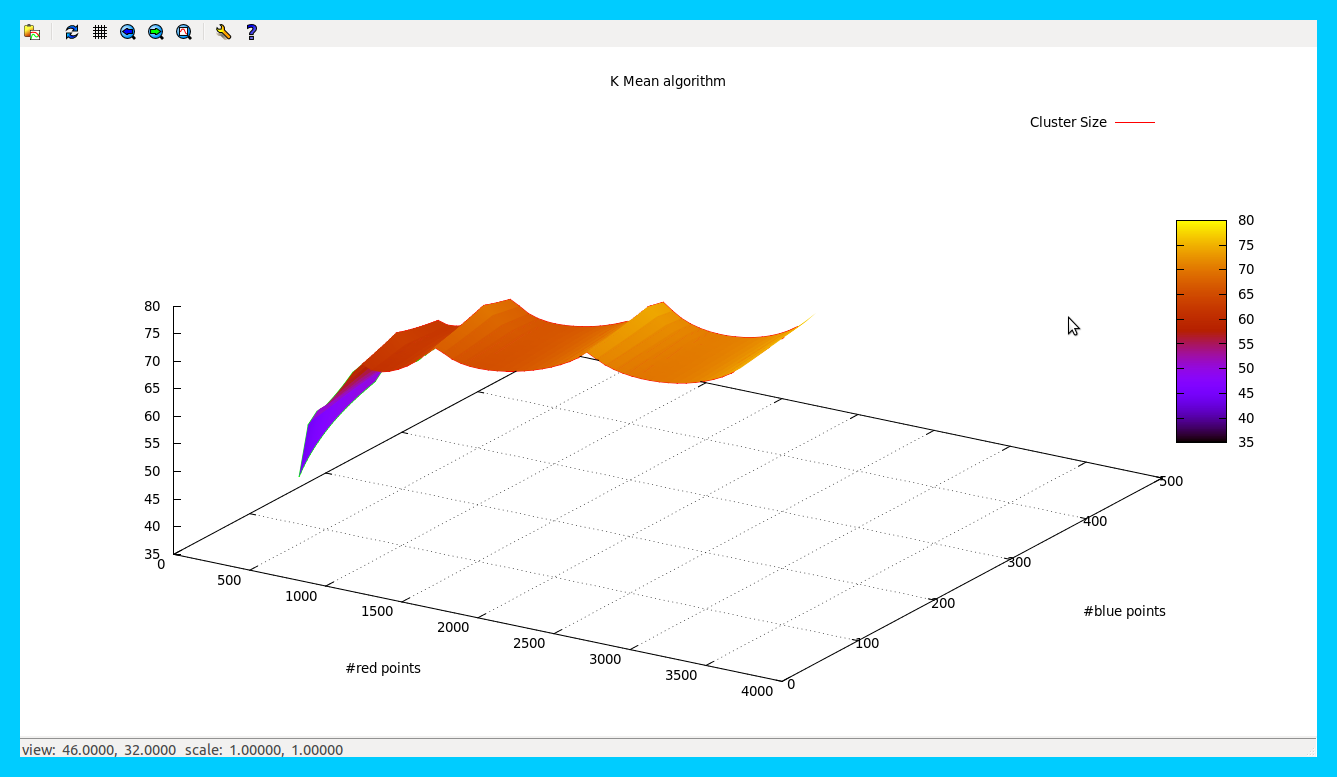
\includegraphics{avg100h.png}}
\end{figure}

%Following results are obtained when a and y varry over interval 1 to 1000.\\ \\
 \begin{table}[H]
\centering
\caption{Results obtained in interval setting domain 1 to 1000 for x and y both}
 \begin{tabular}{||l|c|r||} \hline
 Red Points & Blue Points & K \\ \hline
 0100 & 1485 & 098 \\ \hline
 0200 & 1680 & 194 \\ \hline
 0500 & 2745 & 465 \\ \hline
 0700 & 0071 & 630 \\ \hline
 1000 & 1250 & 867 \\ \hline
 \end{tabular}
 \end{table}
 
\begin{figure}[H]
 \caption{Surface plot for the cluster for interval 1 to 1000}
  \centering
\scalebox{0.3}
{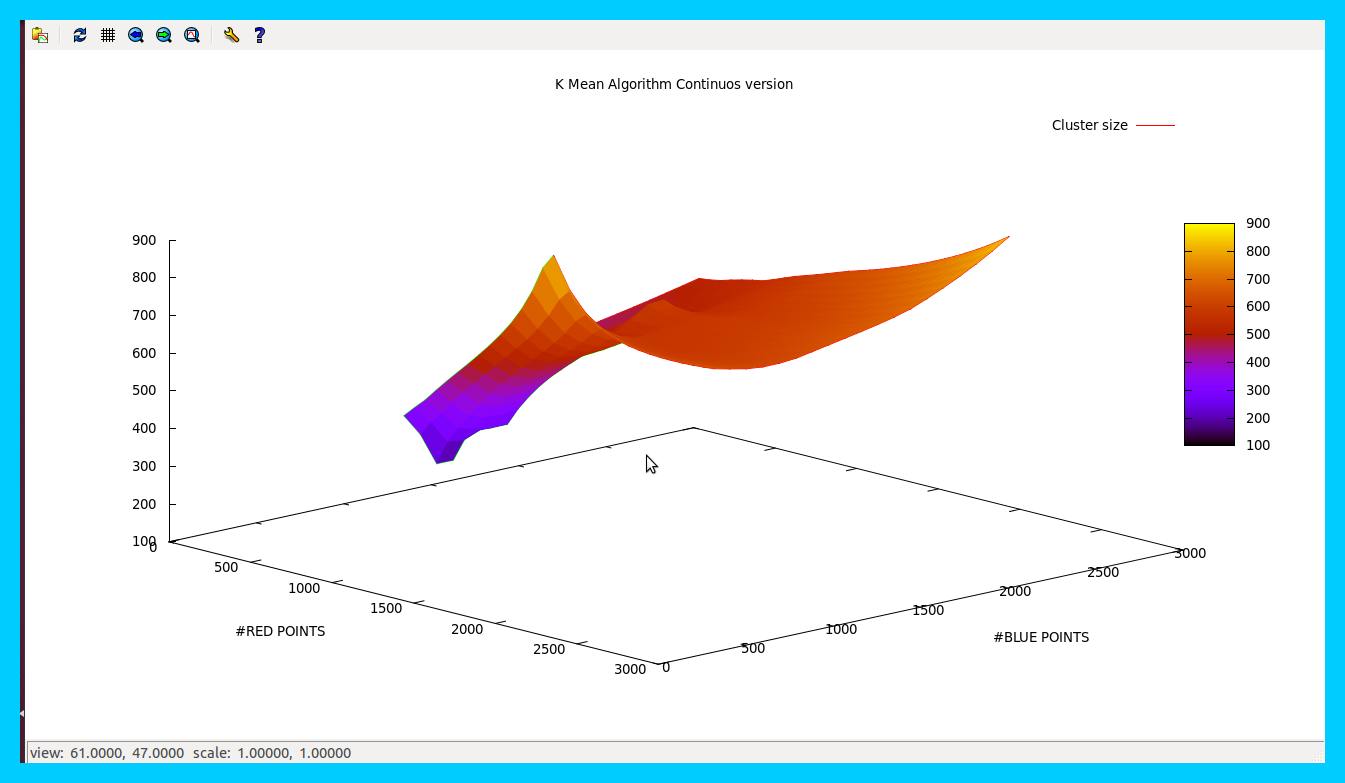
\includegraphics{avg1000.png}}
\end{figure}

 \begin{table}[H]
\centering
\caption{Results obtained in interval setting domain 1 to 100 for x and y both for descrete version of K Mean algorithm}
 \begin{tabular}{||l|c|r||} \hline
 Red Points & Blue Points & K \\ \hline
 100 & 140 & 056 \\ \hline
 200 & 168 & 082 \\ \hline
 500 & 185 & 121 \\ \hline
 700 & 208 & 137 \\ \hline
 1000& 210 & 144 \\ \hline
 \end{tabular}
 \end{table}

 \begin{figure}[H]
 \caption{Surface plot for the cluster for interval 1 to 100}
  \centering
\scalebox{0.3}
{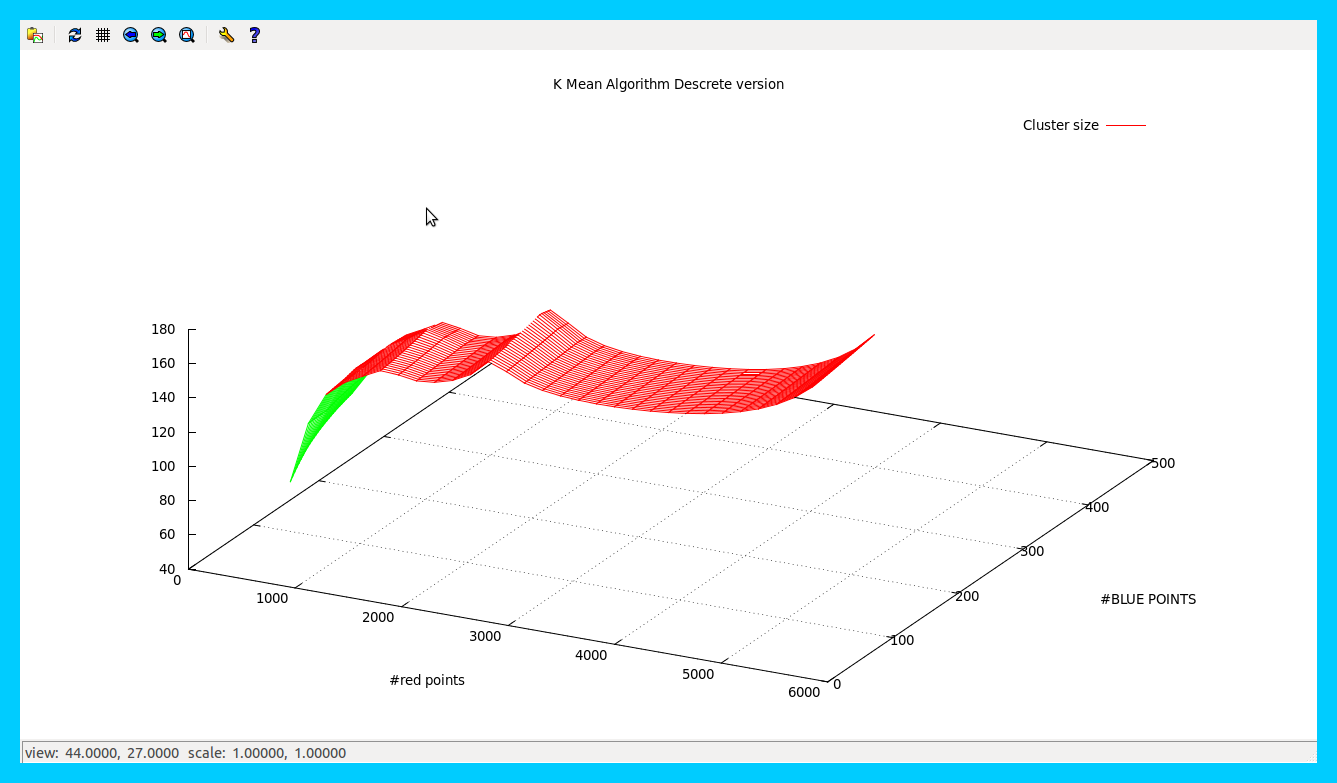
\includegraphics{avg100d.png}}
\end{figure}

\begin{table}[H]
  \centering
  \caption{Variation of radius}
  \begin{tabular}{||l|c|c|c|c||} \hline
   Radius & K & actual K & red points covered \\ \hline
   30.46310 & 010 & 10 & 011 \\ \hline
   23.76970 & 010 & 10 & 013 \\ \hline
   23.76970 & 010 & 10 & 019 \\ \hline \hline
   24.35160 & 025 & 22 & 050 \\ \hline
   20.02500 & 025 & 22 & 060 \\ \hline
   17.00000 & 025 & 22 & 067 \\ \hline
   17.00000 & 025 & 22 & 071 \\ \hline \hline 
   16.27880 & 040 & 31 & 057 \\ \hline
   16.27880 & 040 & 31 & 072 \\ \hline
   16.27880 & 040 & 31 & 075 \\ \hline \hline
   17.20470 & 055 & 37 & 064 \\ \hline
   15.23150 & 055 & 37 & 087 \\ \hline \hline 
   18.97310 & 070 & 40 & 086 \\ \hline
   12.64910 & 070 & 40 & 093 \\ \hline
   12.64910 & 070 & 40 & 096 \\ \hline \hline 
   15.13270 & 085 & 44 & 080 \\ \hline 
   11.31370 & 085 & 44 & 093 \\ \hline 
   11.31370 & 085 & 44 & 095 \\ \hline \hline 
   15.26430 & 100 & 46 & 083 \\ \hline 
   12.08300 & 100 & 46 & 098 \\ \hline \hline 
   12.64910 & 130 & 52 & 095 \\ \hline 
   10.04990 & 130 & 52 & 096 \\ \hline \hline 
   16.27880 & 145 & 53 & 095 \\ \hline 
   15.81140 & 145 & 53 & 096 \\ \hline \hline 
   11.40180 & 160 & 55 & 093 \\ \hline 
   09.48683 & 160 & 55 & 100 \\ \hline \hline 
   
  \end{tabular}
\end{table}

\section{Conclusion}
Both K Mean Continuos Version and K Mean Discrete Version algorithm are able to find the cover. In cases where we have
tremenduosly huge data the convergence rate is slow. Also when the domain is very large then discrete version works better
than continuos version but still both have slow convergence rate. Discrete Version converges faster than continuos version.
 
\clearpage
\bibliographystyle{plain}
\begin{thebibliography}{10} 
 \bibitem{LY94} Lund, Carsten, Yannakakis, Mihalis \textit{On the hardness of approximating minimization problems} J. ACM, 
41, (1994) (960-981)
 \bibitem{GRALB12} Gautam K. Das, Robert Fraser, Alejandro Lopez-Ortiz, and Bradford G. Nickerson 
                \textit{On the descrete unit disk cover problem}. 5th International Workshop, WALCOM 2011, New Delhi, 
                India, February 18-20, 2011. LNCS-6552 (2011) (146-157)
          
 \bibitem{FMS81}Fowler, M. Paterson and S. Tanimoto, \textit{Optimal packing and covering in the plane are np-complete}, Inf. Proc. 
               Let., 12, (1981) (133-137).
 \bibitem{T91}T. Gonzalez, \textit{Covering a set of points in multidimensional space}, Inf. Proc. Let., 40, (1991) (181-188). 
 \bibitem{DW85}D. Hochbaum and W. Maass, \textit{Approximation schemes for covering and packing problems in image processing and VLSI}, 
         J. ACM, 32, (1985) (130-136).
 \bibitem{FGRSR10}F. Claude, G. K. Das, R. Dorrigiv, S. Durocher, R. Fraser, A. Lopez-Ortiz, B. G. Nickerson and A. Salinger, 
                 \textit{An improved line-separable algorithm or discrete unit disk cover}, Disc. Math, Alg. and Appl., 2, (2010) (77-87).
 \bibitem{GSSB}Gautam K. Das, Sandip Das, Subhas C. Nandy, Bhabani P. Sinha, \textit{Efficient Algorithm for placing a given number of base stations to cover a covex
             region}J. Parallel Distrib. Comput. 66 (2006) (1353-1358).


 \end{thebibliography}
 
\end{document}
